

\documentclass{beamer}


% Setup appearance:

\usetheme{Darmstadt}
\usefonttheme[onlylarge]{structurebold}
\setbeamerfont*{frametitle}{size=\normalsize,series=\bfseries}
\setbeamertemplate{navigation symbols}{}


% Standard packages

\usepackage[english]{babel}
\usepackage[latin1]{inputenc}
\usepackage{times}
\usepackage[T1]{fontenc}


% Setup TikZ

\usepackage{ifthenx}
\usepackage{tikz}
\usetikzlibrary{arrows}
\usetikzlibrary{calc}
\usepackage{pgfmath}
\usepackage{verbatim}
\usepackage{listings}
\tikzstyle{block}=[draw opacity=0.7,line width=1.4cm]
\lstset{language=C}

% Author, Title, etc.

\title[Monitor Platform Architecture Specs] 
{%
Monitor Platform Architecture Spec %
}

\author[Sinha N]
{
  Nish~Sinha\inst{1} \and
  Weihong~Wang\inst{1} \and
  Nitul~Jain\inst{1} \and
}

\institute[Xad]
{
  \inst{1}%
  Xad Inc., Mountain View, CA, USA
  \and
  \vskip-2mm
}

\date[\today]
{\today}



% The main document

\newcommand{\drawLinkArrowVertical}[4]{
	\draw[->] let
		\p1 = (#1), \p2 = (#2),
		\p3 = (#3), \p4 = (#4)
		in
		({(\x1 + \x2)*1/2} ,\y1) -- ({(\x3 + \x4)*1/2} ,\y4);
}

\newcommand{\drawLinkArrowHorizontal}[4]{
	\draw[<->] let
		\p1 = (#1), \p2 = (#2),
		\p3 = (#3), \p4 = (#4)
		in
		(\x2, {(\y1 + \y2)*1/2}) -- (\x3, {(\y3 + \y4)*1/2});
}

\newcommand{\drawBox}[5]{{0}
		\shade[top color=#4,bottom color=#4,xslant=#5] (#1) rectangle (#2) node[midway,below] {#3};
}

\begin{document}

\begin{frame}
  \titlepage
\end{frame}

\begin{frame}{Outline}
  \tableofcontents
\end{frame}


\section{The Architecture}

\subsection{The Architecture}

\begin{frame}{Schema}
   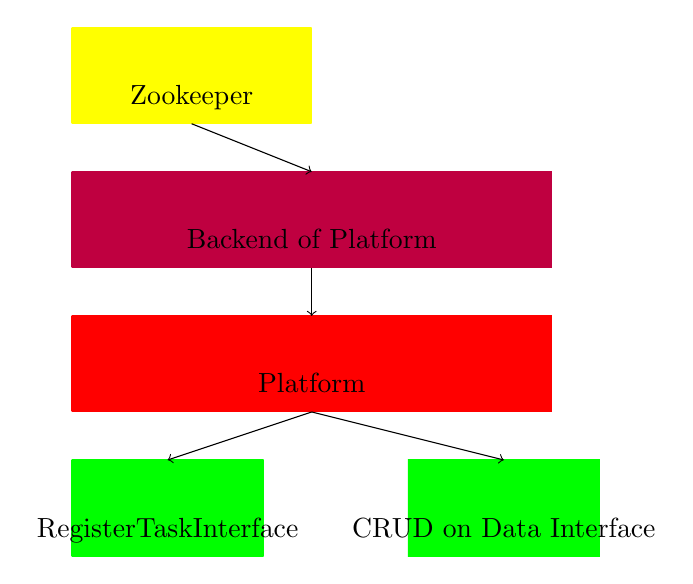
\begin{tikzpicture}[scale=0.61]
	\coordinate (B1_L) at (0,0);
	\coordinate (B1_R) at (5,2);
	\coordinate (B2_L) at (0,-3);
	\coordinate (B2_R) at (10,-1);
	\coordinate (B3_L) at (0,-6);
	\coordinate (B3_R) at (10,-4);
	\coordinate (B4_L) at (0,-9);
	\coordinate (B4_R) at (4,-7);
	\coordinate (B5_L) at (7,-9);
	\coordinate (B5_R) at (11,-7);
	\drawBox{B1_L}{B1_R}{Zookeeper}{yellow}{0}
	\drawBox{B2_L}{B2_R}{Backend of Platform}{purple}{0}
	\drawBox{B3_L}{B3_R}{Platform}{red}{0}
	\drawBox{B4_L}{B4_R}{RegisterTaskInterface}{green}{0}
	\drawBox{B5_L}{B5_R}{CRUD on Data Interface}{green}{0}
	\drawLinkArrowVertical{B1_L}{B1_R}{B2_L}{B2_R}
	\drawLinkArrowVertical{B2_L}{B2_R}{B3_L}{B3_R}
	\drawLinkArrowVertical{B3_L}{B3_R}{B4_L}{B4_R}
	\drawLinkArrowVertical{B3_L}{B3_R}{B5_L}{B5_R}

  \end{tikzpicture}

\end{frame}

\section {RegisterTaskInterface}
\subsection {RegisterTaskInterface}
\begin{frame}
	\begin{block}{RegisterTaskInterface}
		\begin{itemize}
			\item bool \alert{RegisterTask}(Namespace, PlatformTask(initFn,quitFn,runnableMainTask,CallFrequencyConfig)).
			\begin{itemize}
				\item Namespace(name: String, access:Enum\{exclusive, inclusive\}).
				\item CallFrequnecyConfig(Type: Enum\{periodic,watchOnEvent,\textit{dontcallmewillcallyou}\}), period: milliseconds).
			\end{itemize}
		\end{itemize}
	\end{block}
\end{frame}


\section {DataInterface}
\subsection {DataInterface}
\begin{frame}
\begin{block}{DataInterface}
		\begin{itemize}
			\item bool \alert{createData}(key:String,value:String)
			\item bool \alert{updateData}(key:String,value:String)
			\item bool \alert{deleteData}(key:String)
			\item bool \alert{existsData}(key:String)
			\item String \alert{readData}(key:String)
			\item bool \alert{watchData}(key:String, fn: Function)
		\end{itemize}
	\end{block}

\end{frame}


\section {Backend Interface of Platform}
\subsection {Backend Interface of Platform}
\begin{frame}
   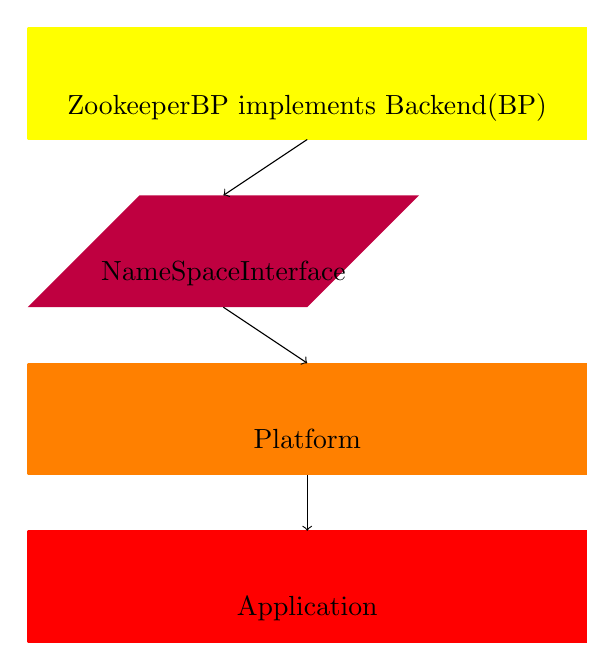
\begin{tikzpicture}[scale=0.71]
     
	\coordinate (B1_L) at (0,0);
	\coordinate (B1_R) at (10,2);
	\coordinate (B2_L) at (0,-3);
	\coordinate (B2_R) at (7,-1);
	\coordinate (B3_L) at (0,-6);
	\coordinate (B3_R) at (10,-4);
	\coordinate (B4_L) at (0,-9);
	\coordinate (B4_R) at (10,-7);

	\drawBox{B1_L}{B1_R}{ZookeeperBP implements Backend(BP)}{yellow}{0}
	\drawBox{B2_L}{B2_R}{NameSpaceInterface}{purple}{1}
	\drawBox{B3_L}{B3_R}{Platform}{orange}{0}
	\drawBox{B4_L}{B4_R}{Application}{red}{0}
	\drawLinkArrowVertical{B1_L}{B1_R}{B2_L}{B2_R}
	\drawLinkArrowVertical{B2_L}{B2_R}{B3_L}{B3_R}
	\drawLinkArrowVertical{B3_L}{B3_R}{B4_L}{B4_R}

  \end{tikzpicture}
\end{frame}


\section {BackendInterface}
\subsection {BackendInterface}
\begin{frame}
\begin{block}{BackendInterface}
		\begin{itemize}
			\item bool \alert{createNamespace}(name:String)
			\item bool \alert{deleteNamespace}(name:String)
			\item bool \alert{setNamespace}(name:String)
			\item bool \alert{exclusiveAccessNamespace}(fn:callbackFn)
			\item bool \alert{inclusiveAccessNamespace}(fn:callbackFn)
			\item bool \alert{createDataNamespace}(key:String)
			\item bool \alert{deleteDataNamespace}(key:String)
			\item bool \alert{watchDataNamespace}(key:String)
			\item String \alert{readDataNamespace}(key:String)
			\item bool \alert{checkDataNamespace}(key:String)
			\item bool \alert{updateDataNamespace}(key:String)
		\end{itemize}
	\end{block}

\end{frame}





\section {Example}
\subsection {Example1}

\begin{frame}{AWS capacity application}
  \begin{example}
	\begin{itemize}
		\item Consists of two tasks: A leader task and a follower task.
			\begin{itemize}
				\item LeadTask is exclusive on the namespace, and node running it is responsible for querying ELB and populating the namespace with relevant data.
				\item FollowTask is inclusive on the namespace, and every node running it is responsible for querying namespace and for maintaining the local cache in coherence. 
				\item \alert{There is no application level coupling between these two tasks. We will see in a later example why that might be important.}.
			\end{itemize}
	\end{itemize}
	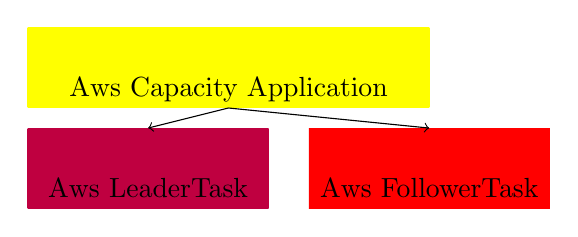
\begin{tikzpicture}[scale=0.51]
		\coordinate (B1_L) at (0,0);
		\coordinate (B1_R) at (10,2);
		\coordinate (B2_L) at (0,-2.5);
		\coordinate (B2_R) at (6,-0.5);
		\coordinate (B3_L) at (7,-2.5);
		\coordinate (B3_R) at (13,-0.5);

		\drawBox{B1_L}{B1_R}{Aws Capacity Application}{yellow}{0}
		\drawBox{B2_L}{B2_R}{Aws LeaderTask}{purple}{0}
		\drawBox{B3_L}{B3_R}{Aws FollowerTask}{red}{0}
		\drawLinkArrowVertical{B1_L}{B1_R}{B2_L}{B2_R}{orange}
		\drawLinkArrowVertical{B1_L}{B1_R}{B3_L}{B3_R}{green}

  	\end{tikzpicture}

  \end{example}
\end{frame}


\begin{frame}[fragile]{AWS capacity application}
	\tiny
	\begin{itemize}
		\item LeaderTask:
	\begin{lstlisting}
	RegisterTask(Namespace(ZK::AWSCAPACITY,
exclusive),new PlatformTask(initFn = () => (),
			quitFn = ()=>(), CallFrequencyConfig(periodic,60000)), 
	def task = ()=> {
	pollAws();
	enumerateActiveNodes();
	foreach node in ActiveNodes :createdata(node,metastate)	
	})
	\end{lstlisting}

	\item FollowerTask:
	\begin{lstlisting}
	RegisterTask(Namespace(ZK::AWSCAPACITY,
inclusive),new PlatformTask(initFn = () => (),
			quitFn = ()=>(), CallFrequencyConfig(watch,-1)), 
	def task = () => {
	x: String= readData(""); //x will contain a list of name of nodes  inside the namespace watched
	updateLocalDataStructures();
})
 
	\end{lstlisting}

	\end{itemize}
\end{frame}


\section {Example2}
\subsection {Example2}
\begin{frame}{Atlantic Health}
  \begin{example}
	\begin{itemize}
		\item Consists of One main task and innumerable dependent task: A system watcher Healthtask.
			\begin{itemize}
				\item HealthTask is inclusive on the namespace, and node running it is responsible for querying the underlying system and placing its health state in namespace.
				\item DependentOnHealthTask is inclusive on some other namespace. It creates special state or takes some special action based on cue from HealthTask as we will see.
			\end{itemize}
	\end{itemize}
	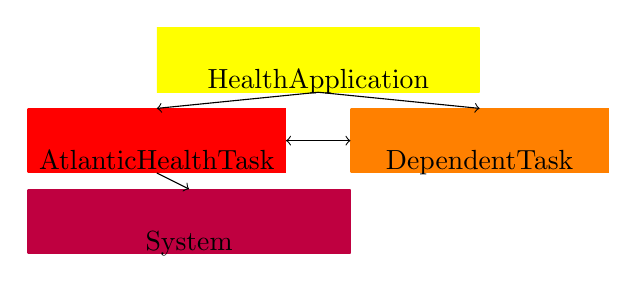
\begin{tikzpicture}[scale=0.41]
		\coordinate (B1_L) at (4,0);
		\coordinate (B1_R) at (14,2);
		\coordinate (B2_L) at (0,-2.5);
		\coordinate (B2_R) at (8,-0.5);
		\coordinate (B3_L) at (0,-5);
		\coordinate (B3_R) at (10,-3);
		\coordinate (B4_L) at (10,-2.5);
		\coordinate (B4_R) at (18,-0.5);

		\drawBox{B1_L}{B1_R}{HealthApplication}{yellow}{0}
		\drawBox{B2_L}{B2_R}{AtlanticHealthTask}{red}{0}
		\drawBox{B4_L}{B4_R}{DependentTask}{orange}{0}
		\drawBox{B3_L}{B3_R}{System}{purple}{0}
		\drawLinkArrowVertical{B1_L}{B1_R}{B2_L}{B2_R}
		\drawLinkArrowVertical{B1_L}{B1_R}{B4_L}{B4_R}
		\drawLinkArrowVertical{B2_L}{B2_R}{B3_L}{B3_R}
		\drawLinkArrowHorizontal{B2_L}{B2_R}{B4_L}{B4_R}

  	\end{tikzpicture}

  \end{example}
\end{frame}

\begin{frame}[fragile]{Atlantic Health}
	\tiny
	\begin{itemize}
		\item HealthTask:
		\begin{lstlisting}
		RegisterTask(Namespace(ZK::ATLANTICHEALTH,
		inclusive),new PlatformTask(initFn = () => (),
			quitFn = ()=>(), CallFrequencyConfig(periodic,60000)), 
		def task = ()=> {
		pollSystem();
		updateData(node,metastate)	
		})
		\end{lstlisting}

		\item DependentTask:
		\begin{lstlisting}
		RegisterTask(Namespace(ZK::DEPENDENTTASK,
	inclusive),new PlatformTask(initFn = () => (),
			quitFn = ()=>(), CallFrequencyConfig(dontcallmewillcallyou,-1)), 
	def task = ()=> {
	getWokenupByHealthApp();	
	updateData(node,metastate)	
	})
	\end{lstlisting}


	\end{itemize}
\end{frame}



\appendix

\section*{Appendix}


\end{document}

